\section{Methodology}\label{sec:method}


\begin{figure*}[!t]
 \centering
 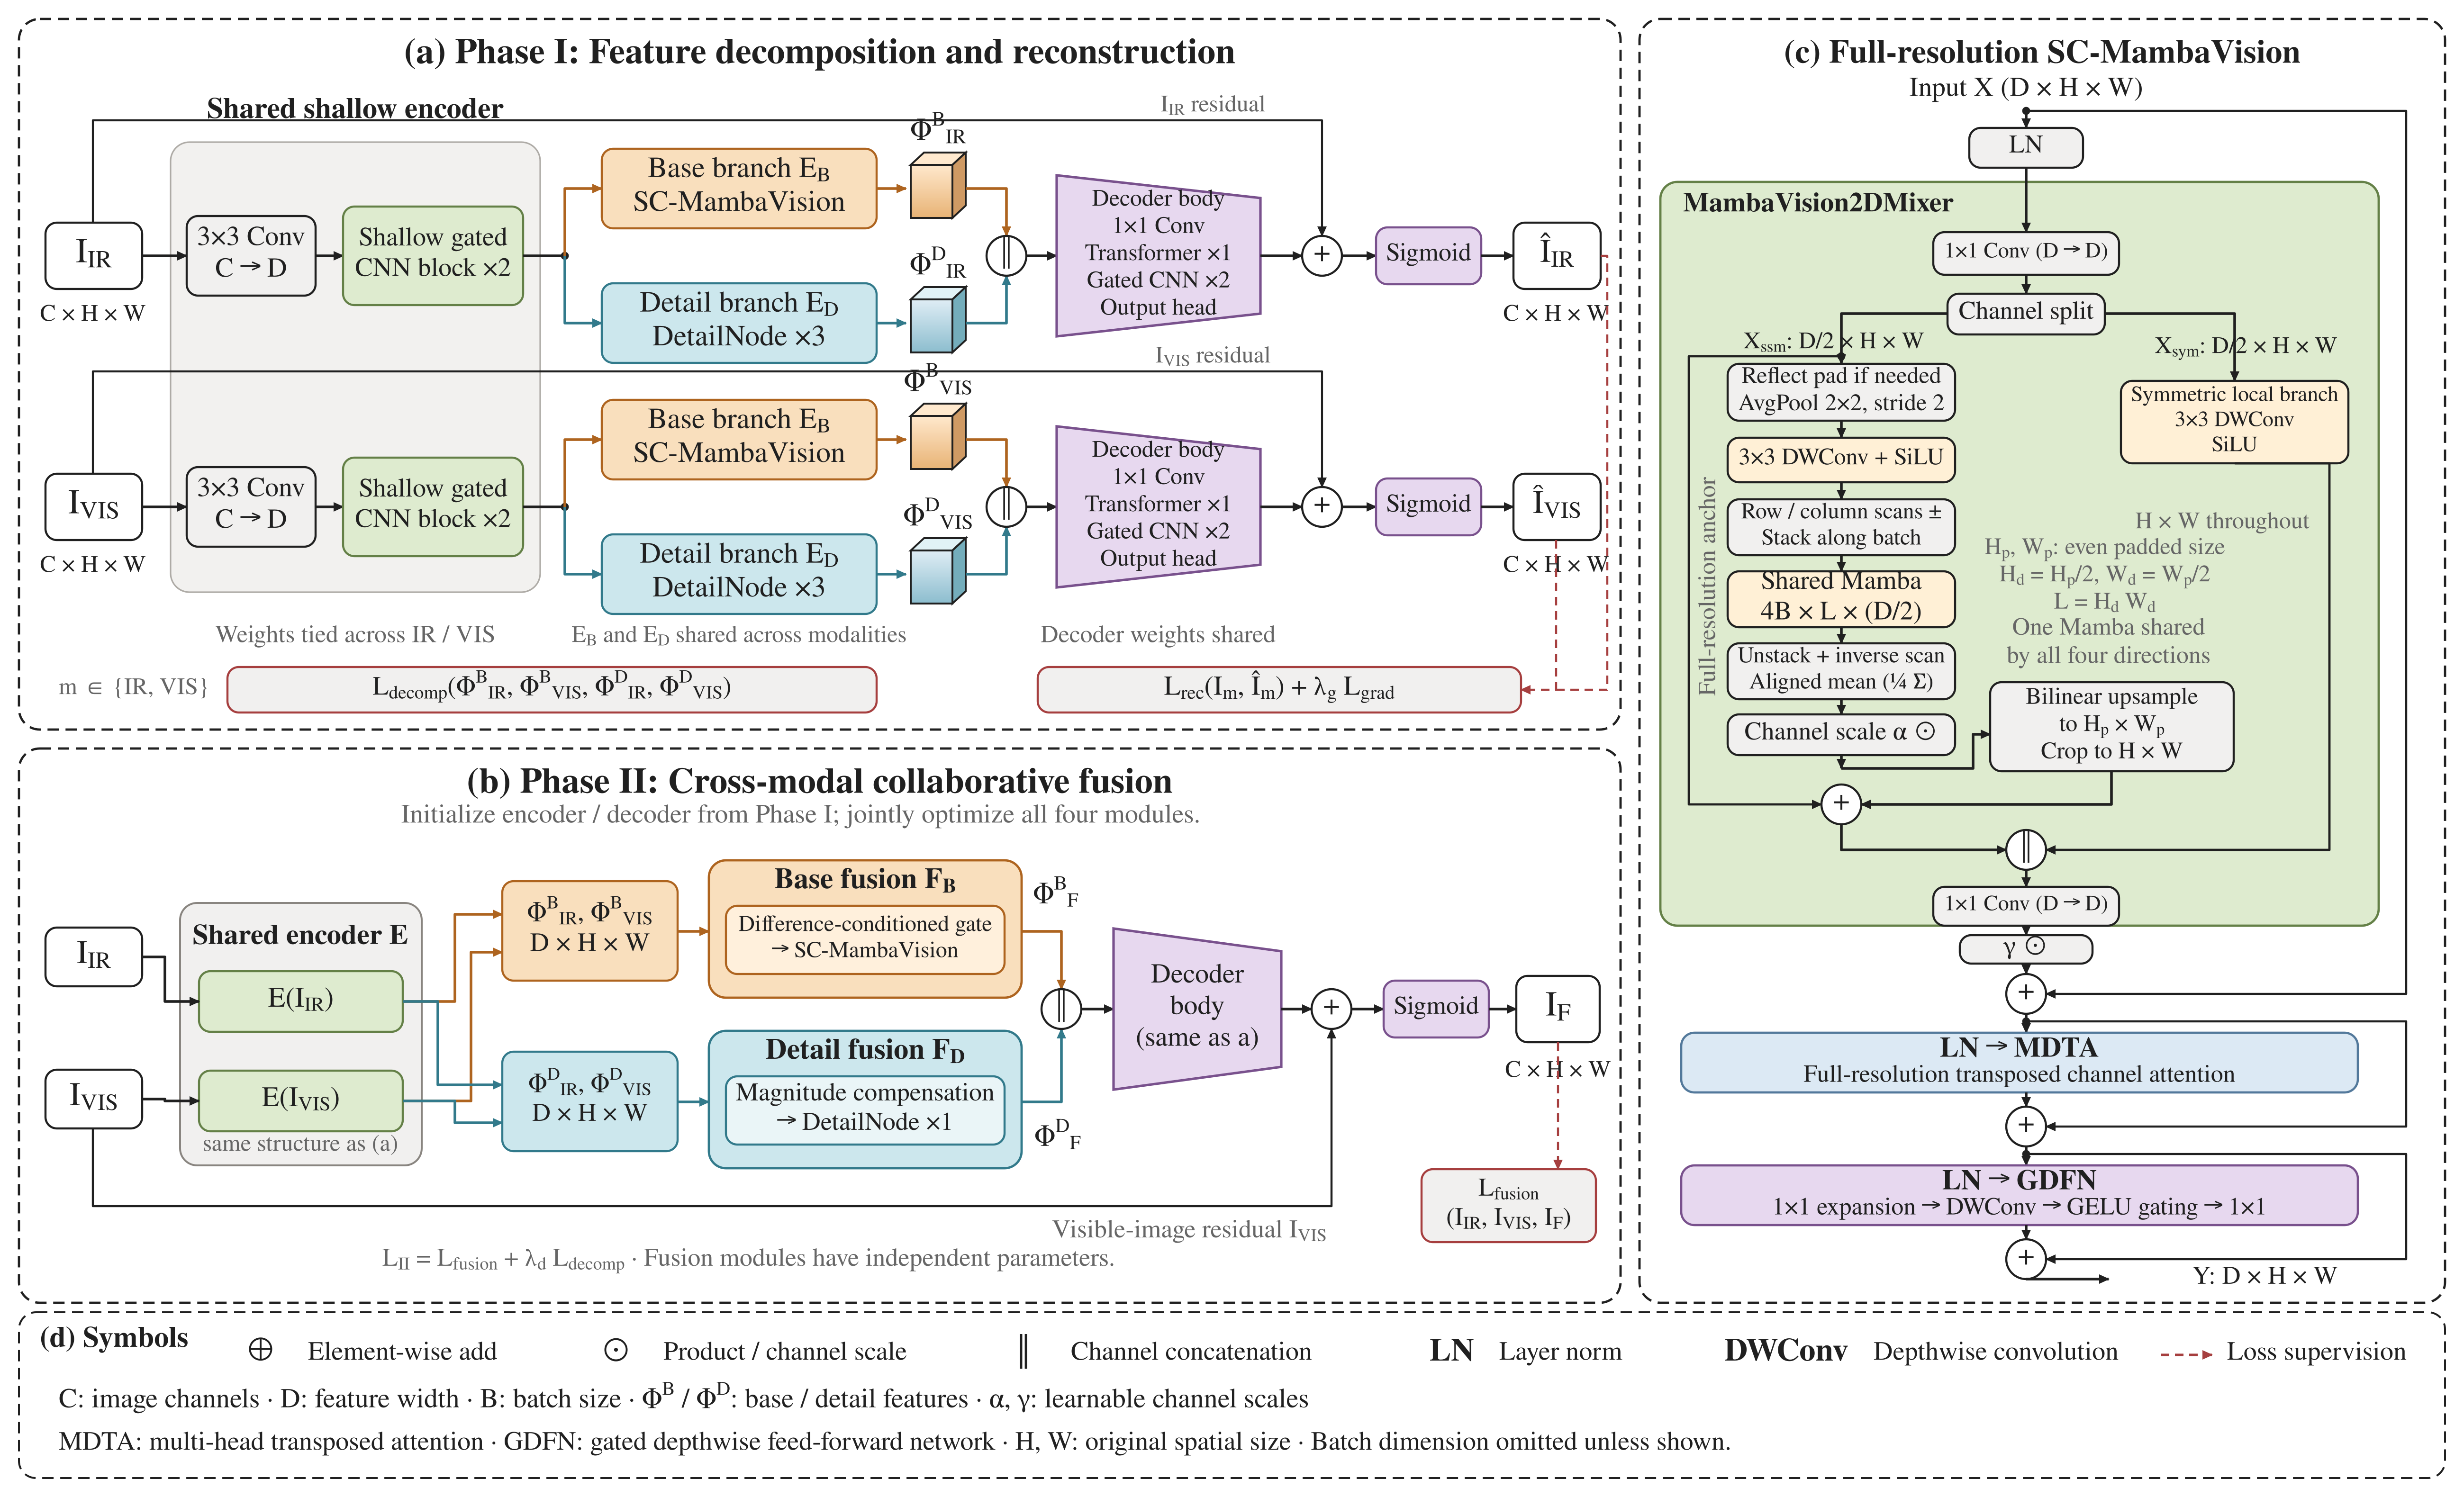
\includegraphics[width=\textwidth]{figs/pipeline.png}
 \caption{Architecture of SCMFuse. (a) Phase I learns base and detail representations by reconstructing each source image with shared encoder and decoder weights. (b) Phase II initializes these components from Phase I and trains cross-modal fusion jointly. (c) The SCM Block combines pooled four-directional scanning, full-resolution residual features, and transposed channel attention. (d) Symbol definitions. The shallow gated CNN block, SC-MambaVision, and MambaVision2DMixer are referred to as SGC Block, SCM Block, and 2D-MV Mixer in the text; base and detail fusion are denoted by DGF and MGF.}
 \label{fig:pipeline}
\end{figure*}

\subsection{Overview}\label{subsec:overall_arch}
Given a registered infrared image $\Iir\in\R^{B\times1\times H\times W}$ and the luminance of a visible image $\Ivis$ with the same dimensions, SCMFuse predicts a fused luminance image $\Ifuse$. Here $B$ is the batch size, $H\times W$ is the spatial resolution, and $D=64$ denotes the feature width. As shown in \cref{fig:pipeline}, the network follows the dual-branch decomposition framework of CDDFuse~\cite{zhao2023cddfuse}:
\begin{equation}
\begin{aligned}
 \Fsh_m&=\Eshared(\mathbf I_m),\\
 (\Fbase_m,\Fdet_m)&=(\Ebase(\Fsh_m),\Edetail(\Fsh_m)),\\
 \Fbase_{\mathrm f}&=\FfuseB(\Fbase_{\mathrm{ir}},\Fbase_{\mathrm{vis}}),\\
 \Fdet_{\mathrm f}&=\FfuseD(\Fdet_{\mathrm{ir}},\Fdet_{\mathrm{vis}}),
\end{aligned}\label{eq:framework}
\end{equation}
where $m\in\{\mathrm{ir},\mathrm{vis}\}$. The encoder and decomposition branches share weights across modalities. Base and detail features are learned representations encouraged to capture shared structure and complementary details; they are not fixed frequency-filter outputs.

We use a \emph{shallow gated convolution block} (\textbf{SGC Block}) for efficient local processing. The base branch uses a \emph{space--channel MambaVision block} (\textbf{SCM Block}), while the detail branch retains the INN-based design of CDDFuse. The fusion layers use \emph{difference-guided fusion} (\textbf{DGF}) for base features and \emph{magnitude-guided fusion} (\textbf{MGF}) for detail features. A hybrid decoder reconstructs the output from the two fused streams. Architectural specifications are summarized in \cref{tab:tensor_dimensions}.

Training has two phases. Phase I learns feature decomposition through source-image reconstruction. Phase II initializes the encoder and decoder from Phase I and learns cross-modal fusion with the proposed supervision. The training phases are distinct from the model configurations evaluated in \cref{subsec:ablation_study}.


\begin{table}[!t]
\centering
\caption{Network specification. All feature maps retain $H\times W$ except inside the scan path. $D=64$; base and detail inputs to the decoder are concatenated.}
\label{tab:tensor_dimensions}
\small
\setlength{\tabcolsep}{3pt}
\begin{tabular}{@{}llc@{}}
\toprule
Component & Main operations & Channels\\
\midrule
Shared encoder & $3\times3$ conv., $2\times$ SGC & $1\to D$\\
Base branch & SCM Block & $D\to D$\\
Detail branch & $3\times$ detail node & $D\to D$\\
Base fusion & DGF, SCM refinement & $2D\to D$\\
Detail fusion & MGF, $1\times$ detail node & $2D\to D$\\
Hybrid decoder & MDTA block, $2\times$ SGC & $2D\to1$\\
\bottomrule
\end{tabular}
\end{table}


\subsection{Efficient Local Processing}
\label{subsec:shallow_encoder}
Full-resolution feature processing is important for dense reconstruction but can account for substantial computation. We use SGC Blocks to capture local patterns with multi-scale depthwise convolutions and retain one transposed-attention block in the decoder to mix base and detail channels. This allocation reduces the repeated attention-based processing used in the baseline encoder and decoder.

\textbf{SGC Block.}
Given $\mathbf X\in\R^{B\times D\times H\times W}$, a point-wise projection expands the normalized features to $2D$ channels and splits them into two streams:
\begin{equation}
 [\mathbf X_a,\mathbf X_b]=\operatorname{Split}
 \big(P_{\mathrm{in}}(\operatorname{LN}(\mathbf X))\big).
\end{equation}
Here $P_{\mathrm{in}}$ is a $1\times1$ convolution and LN denotes layer normalization across channels at each spatial position. The two streams use different kernel sizes:
\begin{equation}
 \mathbf G=\operatorname{SiLU}(\operatorname{DW}_{3}(\mathbf X_a))
              \odot\operatorname{DW}_{5}(\mathbf X_b),
\end{equation}
where $\operatorname{DW}_k$ is a $k\times k$ depthwise convolution and $\odot$ denotes element-wise multiplication. The multiplicative gate combines local responses from the two receptive fields. Channel reweighting and residual refinement then give
\begin{equation}
\begin{aligned}
 \mathbf a&=\sigma\big(P_{\mathrm{ca}}(\operatorname{GAP}(\mathbf G))\big),\\
 \mathbf X'&=\mathbf X+P_{\mathrm{out}}(\mathbf G\odot\mathbf a),\\
 \operatorname{SGC}(\mathbf X)&=\mathbf X'+\operatorname{GDFN}(\operatorname{LN}(\mathbf X')),
\end{aligned}
\end{equation}
where GAP is global average pooling, $P_{\mathrm{ca}}$ and $P_{\mathrm{out}}$ are point-wise convolutions, and $\sigma$ is the sigmoid function. GDFN is the gated depthwise feed-forward network inherited from Restormer~\cite{zamir2022restormer}. A $3\times3$ input convolution followed by two SGC Blocks forms $\Eshared$.

\textbf{Hybrid decoder.}
The decoder concatenates the fused base and detail features and projects them to $D$ channels. It applies one Restormer-style block with multi-DConv head transposed attention (MDTA), followed by two SGC Blocks. The output head contains two $3\times3$ convolutions separated by a LeakyReLU activation. Denoting this reconstruction path by $\mathcal R$, the fused image is
\begin{equation}
 \Ifuse=\sigma\big(\mathcal R([\Fbase_{\mathrm f},\Fdet_{\mathrm f}])+\Ivis\big).
\end{equation}
In Phase I, the same decoder reconstructs each modality using its own source-image residual. The visible residual is used for fusion in Phase II.

\subsection{Space--Channel Base Modeling}\label{subsec:mamba_branch}
MDTA estimates channel relationships from spatially aggregated features, whereas state-space scanning propagates information along spatial sequences. The SCM Block combines these complementary operations. Its residual stream remains at $H\times W$, while pooling is confined to the scanning path.

\textbf{SCM Block.}
For an input feature $\mathbf X$, the block performs
\begin{equation}
\begin{aligned}
 \mathbf X_1&=\mathbf X+\boldsymbol\gamma\odot\mathcal M(\operatorname{LN}(\mathbf X)),\\
 \mathbf X_2&=\mathbf X_1+\operatorname{MDTA}(\operatorname{LN}(\mathbf X_1)),\\
 \operatorname{SCM}(\mathbf X)&=\mathbf X_2+\operatorname{GDFN}(\operatorname{LN}(\mathbf X_2)),
\end{aligned}\label{eq:scm}
\end{equation}
where $\mathcal M$ denotes the two-dimensional MambaVision mixer (\textbf{2D-MV Mixer}) and $\boldsymbol\gamma\in\R^{1\times D\times1\times1}$ is initialized to $0.2$. The base extractor $\Ebase$ uses this block.

\textbf{2D-MV Mixer.}
A point-wise projection splits its input into $\mathbf X_s$ and $\mathbf X_l$, each with $D/2$ channels. The local path processes features at the original resolution:
\begin{equation}
 \mathbf Y_l=\operatorname{SiLU}(\operatorname{DW}_{3}(\mathbf X_l)).
\end{equation}
The spatial path retains $\mathbf X_s$ as an anchor and computes context on a pooled feature map:
\begin{equation}
 \mathbf U=\operatorname{SiLU}\!\left(\operatorname{DW}_{3}
 \big(\operatorname{AvgPool}_{2}(\mathcal P(\mathbf X_s))\big)\right),
\end{equation}
where $\mathcal P$ uses reflection padding to make odd spatial dimensions even. The pooled size is $H_d\times W_d$, with $H_d=\lceil H/2\rceil$ and $W_d=\lceil W/2\rceil$.

The four scan orders are row-major forward/reverse and column-major forward/reverse. Let $\mathcal T_k$ flatten the pooled map in order $k$, and let $\mathcal T_k^{-1}$ restore its spatial layout. All four sequences have length $L=H_dW_d$ and share one Mamba operator~\cite{gu2023mamba}:
\begin{equation}
 \mathbf Y_k=\mathcal T_k^{-1}
 \big(\operatorname{Mamba}(\mathcal T_k(\mathbf U))\big),
 \quad k=1,\ldots,4.
\end{equation}
The directions are stacked along the batch dimension for processing, then spatially aligned and averaged. With a learned channel scale $\mathbf s$, the output is
\begin{equation}
\begin{aligned}
 \mathbf Y_s&=\mathbf X_s+\mathcal U_{H,W}
       \left(\mathbf s\odot\frac14\sum_{k=1}^{4}\mathbf Y_k\right),\\
 \mathcal M(\mathbf X)&=P_{\mathrm m}([\mathbf Y_s,\mathbf Y_l]),
\end{aligned}\label{eq:mixer}
\end{equation}
where $\mathcal U_{H,W}$ uses bilinear interpolation to the padded size and crops to $H\times W$. The learned scale replaces an additional channel normalization at the scan output, leaving relative spatial amplitudes available to subsequent processing.

For even dimensions, each directional sequence has $HW/4$ tokens. The anchor and local path preserve a direct full-resolution route around this pooled computation. MDTA then learns channel interactions from all spatial positions. This combination follows the hybrid modeling motivation of MambaVision~\cite{hatamizadeh2025mambavision}, with directional scanning adapted to image features~\cite{liu2024vmamba}.

\subsection{Difference- and Magnitude-Guided Fusion}
\label{subsec:gated_fusion}
The fusion layers start from additive anchors and learn corrections from cross-modal feature differences. Their refinement modules follow the base and detail branch architectures but use independent weights.

\textbf{DGF for base features.}
Let $\mathbf B_i=\Fbase_{\mathrm{ir}}$ and $\mathbf B_v=\Fbase_{\mathrm{vis}}$. The gate uses both features and their absolute difference:
\begin{equation}
\begin{aligned}
 \mathbf Z_B&=[\mathbf B_i,\mathbf B_v,|\mathbf B_i-\mathbf B_v|],\\
 [\mathbf U_i,\mathbf U_v]&=\mathcal G_B(\mathbf Z_B),\\
 \mathbf W_m&=\mathbf1+\boldsymbol\gamma_B\odot\tanh(\mathbf U_m),
 \quad m\in\{i,v\},\\
 \Fbase_{\mathrm f}&=\operatorname{SCM}_{\mathrm f}
            (\mathbf W_i\odot\mathbf B_i+\mathbf W_v\odot\mathbf B_v).
\end{aligned}
\end{equation}
The gate $\mathcal G_B$ comprises point-wise, depthwise $3\times3$, GELU, and point-wise operations. The shared channel scale $\boldsymbol\gamma_B$ is initialized to $0.1$, so the initial aggregation stays close to addition while allowing modality-dependent corrections.

\textbf{MGF for detail features.}
For $\mathbf D_i=\Fdet_{\mathrm{ir}}$ and $\mathbf D_v=\Fdet_{\mathrm{vis}}$, the magnitude sum provides a cue that remains large when features have opposing signs:
\begin{equation}
\begin{aligned}
 \mathbf Z_D&=[\mathbf D_i,\mathbf D_v,|\mathbf D_i|+|\mathbf D_v|],\\
 \mathbf D_0&=\mathbf D_i+\mathbf D_v+
                  \boldsymbol\gamma_D\odot\mathcal G_D(\mathbf Z_D),\\
 \Fdet_{\mathrm f}&=\operatorname{INN}_1(\mathbf D_0).
\end{aligned}
\end{equation}
Here $\mathcal G_D$ uses the same convolutional pattern as $\mathcal G_B$ with SiLU in place of GELU, and $\boldsymbol\gamma_D$ is initialized to $0.1$. The final refinement uses one detail node, whereas the encoder detail branch contains three nodes. The magnitude cue helps the gate recognize signed-feature disagreement without imposing a fixed sign correction.

\subsection{Training Objectives}\label{subsec:loss_functions}
% Loss primitives: audit/loss_exp4.py. Phase-wise assembly: editorial_review/source_snapshot/models/cddfuse_model.py; configuration: configs/mode/train.yaml in the same snapshot.
The supervision complements reconstruction and cross-modal decomposition with intra-modal decorrelation and image-domain contrast--structure regularization. The new loss components have no trainable inference layers.

\textbf{Feature decorrelation.}
Following CDDFuse, the cross-modal term favors correlated base features and decorrelated detail features. We add an intra-modal penalty:
\begin{equation}
 \Ldecomp=\frac{\CC(\Fdet_{\mathrm{vis}},\Fdet_{\mathrm{ir}})^2}
 {1.01+\CC(\Fbase_{\mathrm{vis}},\Fbase_{\mathrm{ir}})}
 +\lambda_{\mathrm{ortho}}\Lintra.
\end{equation}
The operator $\CC$ is the baseline feature-correlation routine. For each modality, image, and channel, base and detail maps are centered over their spatial positions. With the centered vectors denoted by $\tilde{\mathbf b}_{m,b,c}$ and $\tilde{\mathbf d}_{m,b,c}$, we use
\begin{equation}
 \Lintra=\frac{1}{2BD}\sum_{m,b,c}
 \frac{\langle\tilde{\mathbf b}_{m,b,c},\tilde{\mathbf d}_{m,b,c}\rangle^2}
 {(\|\tilde{\mathbf b}_{m,b,c}\|_2^2+\epsilon)
  (\|\tilde{\mathbf d}_{m,b,c}\|_2^2+\epsilon)}.
\end{equation}
Here $\epsilon=10^{-6}$ and $\lambda_{\mathrm{ortho}}=0.05$. This term discourages redundant spatial patterns between the two representations within each modality.

\textbf{Fusion supervision.}
For $\mathbf M=\max(\Iir,\Ivis)$, the fusion objective is
\begin{equation}
 \Lfusion=\Lin+\lambda_g\Lgrad+
           \lambda_{\mathrm{sd}}\Lsd+\lambda_{\mathrm{struct}}\Lstruct,
 \label{eq:fusion_loss}
\end{equation}
with $\lambda_g=10$, $\lambda_{\mathrm{sd}}=0.5$, and $\lambda_{\mathrm{struct}}=0.12$. We write $\langle\cdot\rangle$ for the mean over the relevant batch, channel, and spatial elements. Intensity and edge supervision retain the source maximum targets:
\begin{equation}
\begin{aligned}
 \Lin&=\langle|\Ifuse-\mathbf M|\rangle,\\
 \Lgrad&=\langle|\mathcal S(\Ifuse)-
                \max(\mathcal S(\Iir),\mathcal S(\Ivis))|\rangle,
\end{aligned}
\end{equation}
where $\mathcal S$ is the Sobel response operator used in the baseline. The additional terms focus on structural agreement and contrast retention.

\textit{Local structural correlation.}
Let $\mathcal A$ be an $11\times11$ mean filter with reflection padding. We compute
\begin{equation}
 \mu_X=\mathcal A(X),\qquad
 s_X=\sqrt{\max(\mathcal A(X^2)-\mu_X^2,0)+\epsilon}.
\end{equation}
For source modality $m$, the stabilized local correlation is
\begin{equation}
 r_{F,m}=\frac{\mathcal A(\Ifuse\mathbf I_m)-\mu_F\mu_m+c_3}
 {s_Fs_m+c_3},\qquad c_3=10^{-4}.
\end{equation}
We weight the modalities by their local standard deviations:
\begin{equation}
 w_{\mathrm{ir}}=\operatorname{sg}\!\left(
 \frac{s_{\mathrm{ir}}}{s_{\mathrm{ir}}+s_{\mathrm{vis}}+10^{-5}}\right),
 \quad w_{\mathrm{vis}}=1-w_{\mathrm{ir}},
\end{equation}
where $\operatorname{sg}$ denotes stop-gradient. The structural loss is
\begin{equation}
 \Lstruct=\big\langle w_{\mathrm{ir}}(1-r_{F,\mathrm{ir}})
              +w_{\mathrm{vis}}(1-r_{F,\mathrm{vis}})\big\rangle.
\end{equation}
This weighting places more emphasis on structural agreement with the source exhibiting greater local intensity variation. Its scale sensitivity is reduced when the stabilizing constants are small relative to the signal statistics.

\textit{Global--local contrast retention.}
Define $g_X=\sqrt{\operatorname{Var}_{HW}(X)+\epsilon}$ using population variance for each image. The reference standard deviations are
\begin{equation}
\begin{aligned}
 t_g&=\operatorname{sg}\!\left[\max\left(g_M,
                 \tfrac12(g_{\mathrm{ir}}+g_{\mathrm{vis}})\right)\right],\\
 t_l&=\operatorname{sg}[\max(s_M,s_{\mathrm{ir}},s_{\mathrm{vis}})].
\end{aligned}
\end{equation}
The contrast loss penalizes values below these references:
\begin{equation}
 \Lsd=\langle\operatorname{ReLU}(t_g-g_F)\rangle
      +\tfrac12\langle\operatorname{ReLU}(t_l-s_F)\rangle.
\end{equation}
The one-sided form encourages contrast retention without forcing the output to match a particular standard deviation above the reference. Intensity and gradient supervision continue to constrain the fused content.


\textbf{Phase-wise optimization.}
Let $\widehat{\mathbf I}_m$ denote a reconstructed source image. Phase I trains the shared encoder and decoder using
\begin{equation}
\begin{aligned}
 \mathcal L_{\mathrm I}
 &=\sum_{m\in\{\mathrm{ir},\mathrm{vis}\}}\mathcal L_{\mathrm{rec},m}
   +2\Ldecomp+5\mathcal L_{\mathrm{rec\text{-}grad}},\\
 \mathcal L_{\mathrm{rec},m}
 &=5\mathcal L_{\mathrm{SSIM}}(\widehat{\mathbf I}_m,\mathbf I_m)
   +\operatorname{MSE}(\widehat{\mathbf I}_m,\mathbf I_m),\\
 \mathcal L_{\mathrm{rec\text{-}grad}}
 &=\sum_m\left\langle\left|
   \nabla\widehat{\mathbf I}_m-\nabla\mathbf I_m\right|\right\rangle.
\end{aligned}\label{eq:phase1_loss}
\end{equation}
Here $\mathcal L_{\mathrm{SSIM}}$ is the mean of $\tfrac12\operatorname{clip}(1-\mathrm{SSIM}_{\mathrm{map}},0,1)$, computed with an $11\times11$ Gaussian window, standard deviation $1.5$, and input range $[0,1]$. The operator $\nabla$ computes spatial gradients. The Gaussian window uses reflection padding. These training operators are distinct from the summed fusion SSIM metric in \cref{subsec:exp_settings}. Phase II jointly optimizes the encoder, decoder, and fusion layers with
\begin{equation}
 \mathcal L_{\mathrm{II}}=\Lfusion+2\Ldecomp.
 \label{eq:phase2_loss}
\end{equation}
For the original-objective configuration Ours-P, the intra-modal and added contrast--structure terms are omitted, and Phase I applies the gradient reconstruction term to the visible image only. Thus, Ours-P and Ours-C differ in supervision during both training phases while retaining the same inference architecture.
% Configuration weights are taken from the archived training caller/configuration. Their association with the reported historical checkpoints still requires the saved run configuration.
